\let\negmedspace\undefined
\let\negthickspace\undefined
\documentclass[journal,12pt,twocolumn]{IEEEtran}
\usepackage{setspace}
\usepackage{amssymb}
\usepackage{graphicx}
\usepackage[cmex10]{amsmath}
\usepackage{amsthm}
\usepackage{enumitem}
\usepackage{mathtools}

\usepackage{listings}
    \usepackage{color}                                            %%
    \usepackage{array}                                            %%
    \usepackage{longtable}                                        %%
    \usepackage{calc}                                             %%
    \usepackage{multirow}                                         %%
    \usepackage{hhline}                                           %%
    \usepackage{ifthen}                                           %%
    \usepackage{lscape}     

\DeclareMathOperator*{\equals}{=}

\renewcommand\thesection{\arabic{section}}
\renewcommand\thesubsection{\thesection.\arabic{subsection}}
\renewcommand\thesubsubsection{\thesubsection.\arabic{subsubsection}}

\renewcommand\thesectiondis{\arabic{section}}
\renewcommand\thesubsectiondis{\thesectiondis.\arabic{subsection}}
\renewcommand\thesubsubsectiondis{\thesubsectiondis.\arabic{subsubsection}}

\let\vec\mathbf                                %%

\lstset{
%language=C,
frame=single, 
breaklines=true,
columns=fullflexible
}
\begin{document}

\bibliographystyle{IEEEtran}

\newcommand{\solution}{\noindent \textbf{Solution: }}
\newcommand{\myvec}[1]{\ensuremath{\begin{pmatrix}#1\end{pmatrix}}}
\newcommand{\mydet}[1]{\ensuremath{\begin{vmatrix}#1\end{vmatrix}}}

\let\vec\mathbf

\vspace{3cm}
\title{
   ASSIGNMENT-1
}
\author{CS21BTECH11024 - Varshini  Jonnala}	

\maketitle

\bigskip
\renewcommand{\thefigure}{\theenumi}
\renewcommand{\thetable}{\theenumi}

\numberwithin{equation}{section}
\numberwithin{figure}{section}
\numberwithin{table}{section}
\section*{ICSE 10 2018 - Problem 7(c)}
\numberwithin{equation}{enumi}
\numberwithin{figure}{enumi}

\begin{center}
    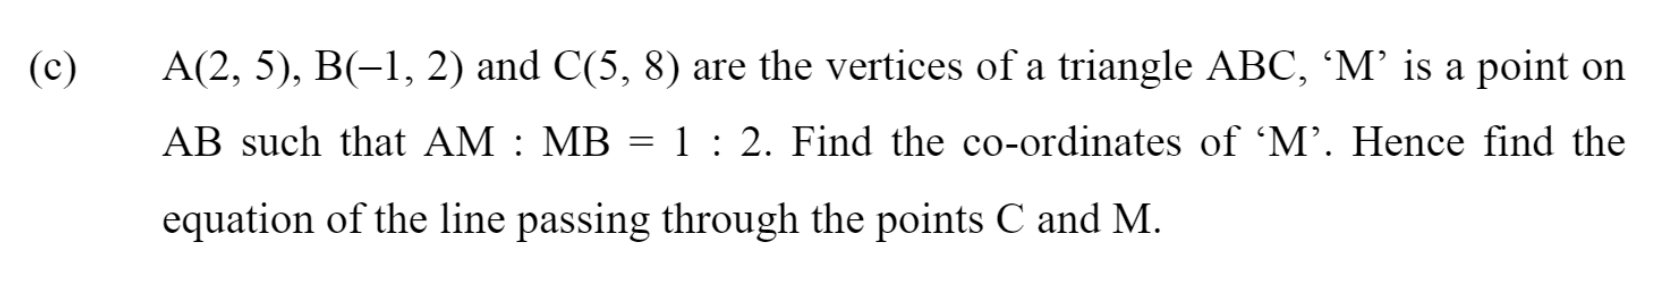
\includegraphics[width=0.49\textwidth]{prv1a.png}
\end{center}

\solution According to the question, $M$ is a point on the side $AB$ such that $$AM : MB = 1 : 2$$
 When the line segment AB is divided internally by C in the ratio $m:n$, from Section formula,\\
 we get the Coordinates of point C as,
\begin{align*}
 \myvec{\frac{mx2+nx1}{m+n}\\\\ \frac{my2+ny1}{m+n}}, where\\
     \vec{A}=\myvec{x1\\y1}, \vec{B}=\myvec{x2\\y2}
\end{align*}
From given data, using Section formula, we get
\begin{align*}
    \vec{M} &= \myvec{\frac{-1+4}{1+2}\\ \frac{2+10}{1+2}}\\ 
    &= \myvec{1\\4}
\end{align*}\\\\\\
The equation of the line joining two points \myvec{a\\b} and \myvec{c\\d} is 
\begin{align*}
    \myvec{y-b} = {\myvec{\frac{d-b}{c-a}}}\myvec{x-a}
\end{align*}
Here, the equation of the line joining points C\myvec{5\\8} and M\myvec{1\\4} will be
\begin{align*}
    \myvec{y-4} = \myvec{\frac{8-4}{5-1}}\myvec{x-1} 
\end{align*}
Simplified, we get the equation
\begin{align*}
    \myvec{1 & - 1}\vec{x} + 3 &=0 
\end{align*}
 which can also be represented as $$x-y+3=0$$
\subsection*{But, However,} On calculating, we get\\
\begin{enumerate}
    \item The equation of the line joining $\vec{A}\myvec{2\\5}, \vec{B}\myvec{-1\\2}$ as $\myvec{1 & - 1}\vec{x} + 3 = 0$ \\\\
    
    \item and the equation of the line joining $\vec{B}\myvec{-1\\2}, \vec{C}\myvec{5\\8}$ as $\myvec{1 & - 1}\vec{x} + 3 = 0$ too.\\

\end{enumerate}

 This implies that $A,B,C$ points are `collinear' and lie on the line $x-y+3=0$ and Hence, given points $A,B,C$ don't form a triangle.\newline\\
Verified by plotting the graph of A,B,C and M points :
\begin{center}
  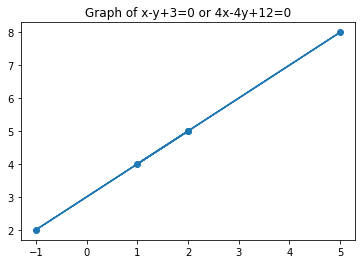
\includegraphics[scale=0.6]{prv1b.png}
\end{center}
    
\end{document}
